\section{期望}
\label{sec:rvm-expectation}

骰子游戏平均能拿多少钱？这个问题要求用一个数概括整张概率表，而且这个数应当按概率给各个取值加权。取值只有有限个时，加权平均就是一个有限和；取值有可数无穷个或由密度给出时，有限和变成级数或积分，就必须先检查它是否有意义。本节先给出定义和存在条件，再建立运算规则，然后说明怎样直接计算函数的平均，最后比较“先平均再变换”与“先变换再平均”。

\subsection{定义}
\label{sec:rvm-expectation-definition}

\paragraph{有限个取值}
设想把骰子游戏玩$6000$次。按概率，大约有$3000$次拿到$0$元，$2000$次拿到$3$元，$1000$次拿到$6$元。总奖金约为
\[
 0\times3000+3\times2000+6\times1000=12000,
\]
平均每次约$2$元。把次数换成比例，这个计算就是按概率加权：
\[
 0\times\tfrac12+3\times\tfrac13+6\times\tfrac16=2 .
\]
重复次数越多，实际平均为什么越接近这个加权和，是第~\ref{chap:laws-of-large-numbers}章大数律的内容。这里只把加权和本身作为定义的出发点，它只用到概率表，与任何一次具体的试验结果无关。

另一种看法来自力学。把总质量$1$按概率分配到数轴上：位置$0$放质量$\tfrac12$，位置$3$放$\tfrac13$，位置$6$放$\tfrac16$。在位置$c$处支起数轴，各质量对支点的力矩之和是$\sum_i(x_i-c)p_X(x_i)$，它等于零时数轴平衡。解出的$c$正是加权和$\sum_ix_ip_X(x_i)=2$。所以加权平均就是这组质量的重心，见图~\ref{fig:rvm-balance}(a)。

\begin{BookInlineFigure}
 \centering
 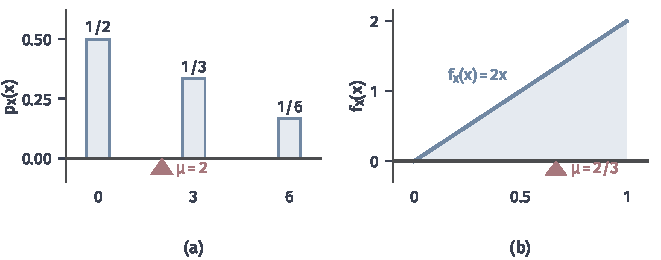
\includegraphics[width=112mm]{figures/07-probability/01-elementary-probability/matplotlib/rvm-balance/figure.pdf}
 \caption{期望是概率质量的重心。(a)奖金表：位置$0,3,6$上分别放质量$\tfrac12,\tfrac13,\tfrac16$（蓝色柱），红色三角是使数轴平衡的支点$\mu=2$，它不是$X$的任何可能取值。(b)密度$f_X(x)=2x$把质量连续地铺在$(0,1)$上，右侧更重，重心在$\mu=2/3$。}
 \label{fig:rvm-balance}
\end{BookInlineFigure}

这个例子说明期望不必是随机变量能取到的值。没有哪一次游戏恰好得$2$元，$2$描述的是质量的平衡位置，而不是某次的典型结果。图中重心偏向左侧，因为一半的质量堆在$0$上；位置$6$虽远，质量却只有$\tfrac16$。

\begin{definition}[有限取值的期望]
\label{def:rvm-expectation-finite}
设随机变量$X$只取有限个值$x_1,\dots,x_n$，概率质量为$p_X(x_i)$。称
\begin{equation}
 \mathbb{E}[X]=\sum_{i=1}^{n}x_i\,p_X(x_i)
 \label{eq:rvm-mean-finite}
\end{equation}
为$X$的\term{期望}（expectation），也称\term{均值}（mean），常记作$\mu$或$\mu_X$。
\end{definition}

\paragraph{从样本点求和}
式~\eqref{eq:rvm-mean-finite}按$X$的取值分组求和。也可以回到试验本身，逐个样本点相加。骰子有六个等可能的点数$\omega=1,\dots,6$，奖金是点数的函数$X(\omega)$。逐点相加得到
\[
 \sum_{\omega=1}^{6}X(\omega)\,\mathbb{P}(\{\omega\})
 =\tfrac16(0+0+0+3+3+6)=2,
\]
与按取值分组的结果相同。图~\ref{fig:rvm-reward-map}显示了这两种算法的关系：先把映到同一个值的样本点归成一组，组内概率之和就是这个值的概率质量。

\begin{BookInlineFigure}
 \centering
 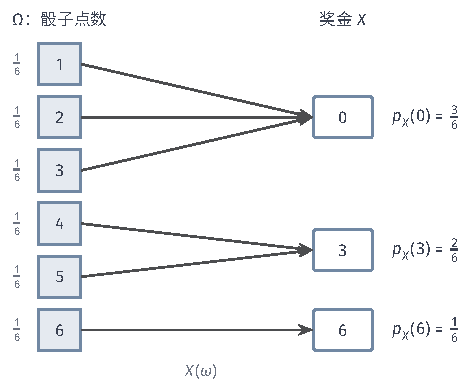
\includegraphics[width=80mm]{figures/07-probability/01-elementary-probability/tikz/rvm-reward-map/figure.pdf}
 \caption{奖金$X$是样本空间$\Omega=\{1,\dots,6\}$上的函数。左侧每个点数的概率是$\tfrac16$；映到同一奖金的点数合成一组，组内概率相加就得到右侧的概率质量。逐点求和与按取值分组求和只是加法的次序不同。}
 \label{fig:rvm-reward-map}
\end{BookInlineFigure}

一般地，若样本空间$\Omega$有限，按$X$的取值把样本点分组，就有
\begin{equation}
 \mathbb{E}[X]=\sum_{\omega\in\Omega}X(\omega)\,\mathbb{P}(\{\omega\}) .
 \label{eq:rvm-mean-sample-points}
\end{equation}
理由是每个样本点恰好落在一组中，而第$i$组的概率之和是$p_X(x_i)$，组内各项的$X(\omega)$都等于$x_i$。有限和可以任意分组与交换次序，所以两种求和结果相同。下一小节将用式~\eqref{eq:rvm-mean-sample-points}证明期望的线性性。

\paragraph{可数个取值}
取值有可数无穷个时，加权和成为级数，这时会出现有限和没有的两个问题：级数可能发散，也可能只在某种求和次序下收敛。先看非负的情形。设$X$取正整数，
\[
 p_X(k)=\frac{1}{k(k+1)},\qquad k=1,2,\dots .
\]
由$\frac{1}{k(k+1)}=\frac1k-\frac1{k+1}$，前$n$项之和是$1-\frac1{n+1}$，它趋于$1$，所以这是一张合法的概率表。

计算加权和时，各项为$k\,p_X(k)=\frac{1}{k+1}$，于是部分和
\[
 \sum_{k=1}^{n}k\,p_X(k)=\sum_{k=1}^{n}\frac{1}{k+1}
\]
随$n$无限增大，增长速度与$\ln n$相同，见图~\ref{fig:rvm-truncated-sums}(a)。各项都非负，部分和单调增加，所以无论按什么次序相加，结果都是$+\infty$。对非负随机变量，这样的结论有明确含义：平均没有上限，我们写$\mathbb{E}[X]=+\infty$。用重心的语言说，质量$\frac{1}{k(k+1)}$随距离$k$衰减得不够快，远处的质量对力矩的贡献加起来没有上界，数轴在任何位置都无法平衡。

有正有负的取值则不同。若正负两部分的加权和都是$+\infty$，部分和的极限取决于正项与负项轮流加入的方式。由级数重排定理，条件收敛的级数重排后可以收敛到任意指定的值，可参考\BookChapterRef{chap:limits-continuity}{卷一第5章“极限与连续”}。概率表里的取值并没有天然的先后次序，所以只有与次序无关的和才适合作为期望。解决办法是把正负两部分分开计算。

\paragraph{正部与负部}
对实数$x$，记$x^{+}=\max\{x,0\}$，$x^{-}=\max\{-x,0\}$，则
\begin{equation}
 x=x^{+}-x^{-},\qquad \lvert x\rvert=x^{+}+x^{-} .
 \label{eq:rvm-pos-neg}
\end{equation}
对随机变量逐个取值使用这两个函数，得到两个非负随机变量$X^{+}$与$X^{-}$，分别称为$X$的\term{正部}（positive part）与\term{负部}（negative part）。$X^{+}$只记录收益，$X^{-}$只记录损失，两者都非负，它们的加权和总有意义，可能是有限数，也可能是$+\infty$。

\paragraph{密度的情形}
有密度时，概率质量连续地铺在数轴上，单位长度上的质量是$f_X(x)$。把小区间$[x,x+\mathrm{d}x]$上的质量$f_X(x)\,\mathrm{d}x$看作放在$x$处，加权和就变成积分。对贯穿例子$f_X(x)=2x$（$0<x<1$），有
\[
 \int_0^1x\cdot2x\,\mathrm{d}x=\left[\tfrac23x^{3}\right]_0^1=\tfrac23 .
\]
图~\ref{fig:rvm-balance}(b)中质量向右堆积，重心落在$2/3$，比区间中点$1/2$偏右。

密度的支撑无界时，积分是反常积分，同样要分正负两部分检查。考虑对称的密度
\[
 f_X(x)=\frac{1}{2x^{2}},\qquad \lvert x\rvert\geq1 .
\]
它在$[1,\infty)$与$(-\infty,-1]$上各有质量$\tfrac12$，总质量为一。正部的积分是
\[
 \int_1^{\infty}x\cdot\frac{1}{2x^{2}}\,\mathrm{d}x=\frac12\int_1^{\infty}\frac{\mathrm{d}x}{x}=+\infty,
\]
负部同理也是$+\infty$。

两侧都无穷时，截断的方式决定了截断后的积分。在$[-a,b]$（$a,b\geq1$）上，正负两侧的贡献分别是$\frac12\ln b$与$-\frac12\ln a$，所以截断积分为$\frac12\ln(b/a)$。对称截断$b=a$得$0$，截断$b=2a$恒得$\frac12\ln2\approx0.35$，截断$b=a^{2}$得$\frac12\ln a\to+\infty$。图~\ref{fig:rvm-truncated-sums}(b)画出了这三种截断。密度关于$0$对称，却不能因此说期望是$0$：期望根本没有定义。

\begin{BookInlineFigure}
 \centering
 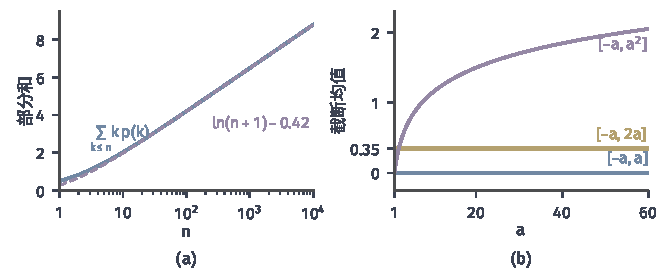
\includegraphics[width=112mm]{figures/07-probability/01-elementary-probability/matplotlib/rvm-truncated-sums/figure.pdf}
 \caption{无穷的加权和。(a)概率表$p_X(k)=1/[k(k+1)]$的部分和$\sum_{k\leq n}k\,p_X(k)$（蓝）与$\ln(n+1)-0.42$（紫色虚线）几乎重合，趋于$+\infty$。(b)对称密度$1/(2x^{2})$（$\lvert x\rvert\geq1$）在$[-a,b]$上的截断积分$\frac12\ln(b/a)$：对称截断（蓝）恒为$0$，$b=2a$（黄）恒为$0.35$，$b=a^{2}$（紫）无界增长。}
 \label{fig:rvm-truncated-sums}
\end{BookInlineFigure}

\paragraph{期望的定义}
上面的例子给出了三种情形：非负变量的加权和总有意义，可能为$+\infty$；有正有负时，只要正负两部分不同时为无穷，差仍有意义；两部分都无穷时没有合理的值。下面的定义同时覆盖概率表与密度。

\begin{definition}[期望]
\label{def:rvm-expectation}
设$X$是取有限或可数个值$x_i$的离散随机变量，概率质量为$p_X$；或$X$有密度$f_X$。$X$的正部与负部的期望定义为
\begin{equation}
 \begin{aligned}
 \mathbb{E}[X^{+}]&=\sum_{x_i>0}x_i\,p_X(x_i)\quad\text{或}\quad\int_0^{\infty}x\,f_X(x)\,\mathrm{d}x,\\
 \mathbb{E}[X^{-}]&=\sum_{x_i<0}(-x_i)\,p_X(x_i)\quad\text{或}\quad\int_{-\infty}^{0}(-x)\,f_X(x)\,\mathrm{d}x,
 \end{aligned}
 \label{eq:rvm-mean-parts}
\end{equation}
它们取值于$[0,+\infty]$。若两者不同时为$+\infty$，定义
\begin{equation}
 \mathbb{E}[X]=\mathbb{E}[X^{+}]-\mathbb{E}[X^{-}] .
 \label{eq:rvm-mean-general}
\end{equation}
若两者都有限，等价地
\begin{equation}
 \mathbb{E}\lvert X\rvert=\mathbb{E}[X^{+}]+\mathbb{E}[X^{-}]<\infty,
 \label{eq:rvm-integrable}
\end{equation}
称$X$\term{可积}（integrable），这时期望是有限实数，并且
\begin{equation}
 \mathbb{E}[X]=\sum_{i}x_i\,p_X(x_i)\quad\text{或}\quad\mathbb{E}[X]=\int_{-\infty}^{\infty}x\,f_X(x)\,\mathrm{d}x,
 \label{eq:rvm-mean-sum-integral}
\end{equation}
其中级数按任何次序求和都绝对收敛，积分是绝对收敛的反常积分。
\end{definition}

定义中三层条件各起不同作用。非负变量的期望总存在，只是可能为$+\infty$，例如$p_X(k)=1/[k(k+1)]$的$X$。有符号变量需要检查正负两部分，只有一侧无穷时期望是$+\infty$或$-\infty$，两侧都无穷时期望不存在，例如上面的对称密度。说“期望有限”或“$X$可积”都要求$\mathbb{E}\lvert X\rvert<\infty$，绝对收敛保证了式~\eqref{eq:rvm-mean-sum-integral}与求和次序、截断方式都无关。

只取有限个值的变量总是可积的，定义~\ref{def:rvm-expectation}在这时就回到式~\eqref{eq:rvm-mean-finite}。取值有界的变量也总是可积：若$\lvert X\rvert\leq M$，则$\mathbb{E}\lvert X\rvert\leq M$。期望可能不存在的情形都来自远处的质量，第~\ref{chap:common-distributions}章会在具体的分布中再次遇到这种现象。

\paragraph{兼有点质量与密度的模型}
有的模型同时含有点质量和连续部分，例如等待时间以概率$0.3$恰为$0$，其余概率$0.7$按密度$0.7\,\mathrm{e}^{-t}$（$t>0$）分布。这时把两部分的贡献相加，
\[
 \mathbb{E}[T]=0\times0.3+\int_0^{\infty}t\cdot0.7\,\mathrm{e}^{-t}\,\mathrm{d}t=0.7 .
\]
这种加法与定义~\ref{def:rvm-expectation}的精神一致，但概率表和密度都不能单独描述这类分布。对一般分布统一的期望定义要借助概率空间上的积分，在第~\ref{chap:probability-spaces}章完成。本部分只用离散求和、密度积分以及两者之和。

\subsection{基本性质}
\label{sec:rvm-expectation-properties}

两个游戏的奖金之和平均是多少？如果期望能逐项相加，只需分别知道两个平均；若不能，就得先求和的完整分布。下面的性质说明，在可积条件下期望对线性组合可以逐项计算，而且不需要任何独立性假设。

\paragraph{线性性、保序性与绝对值估计}
为了让多个随机变量同时有意义，设它们定义在同一个样本空间$\Omega$上。这里先在$\Omega$有限或可数、每个样本点有概率$\mathbb{P}(\{\omega\})$的情形证明，此时期望可以像式~\eqref{eq:rvm-mean-sample-points}那样逐点求和。对可数的$\Omega$，$X$可积等价于$\sum_{\omega}\lvert X(\omega)\rvert\,\mathbb{P}(\{\omega\})<\infty$，按取值分组的论证与有限情形相同，只是用到了绝对收敛级数可以任意分组。

\begin{theorem}[期望的基本性质]
\label{thm:rvm-expectation-properties}
设$X,Y$是同一样本空间上的可积随机变量，$a,b,c$为实数。
(1)线性性：$aX+bY+c$可积，且
\begin{equation}
 \mathbb{E}[aX+bY+c]=a\,\mathbb{E}[X]+b\,\mathbb{E}[Y]+c .
 \label{eq:rvm-linearity}
\end{equation}
(2)保序性：若对每个样本点$X(\omega)\leq Y(\omega)$，则$\mathbb{E}[X]\leq\mathbb{E}[Y]$。
(3)绝对值估计：
\begin{equation}
 \lvert\mathbb{E}[X]\rvert\leq\mathbb{E}\lvert X\rvert .
 \label{eq:rvm-abs-bound}
\end{equation}
\end{theorem}

\begin{proof}
在$\Omega$有限或可数时证明。记$q(\omega)=\mathbb{P}(\{\omega\})$。

线性性。由三角不等式，对每个$\omega$有
\[
 \lvert aX(\omega)+bY(\omega)+c\rvert\leq\lvert a\rvert\,\lvert X(\omega)\rvert+\lvert b\rvert\,\lvert Y(\omega)\rvert+\lvert c\rvert .
\]
两边乘$q(\omega)$后求和，右边是$\lvert a\rvert\,\mathbb{E}\lvert X\rvert+\lvert b\rvert\,\mathbb{E}\lvert Y\rvert+\lvert c\rvert<\infty$，所以$aX+bY+c$可积。三个绝对收敛级数可以逐项相加，于是
\[
 \begin{aligned}
 &\sum_{\omega}\bigl(aX(\omega)+bY(\omega)+c\bigr)q(\omega)\\
 &\quad=a\sum_{\omega}X(\omega)q(\omega)+b\sum_{\omega}Y(\omega)q(\omega)+c\sum_{\omega}q(\omega),
 \end{aligned}
\]
最后一个和等于$1$，这就是式~\eqref{eq:rvm-linearity}。

保序性。$Y-X$在每个样本点非负，所以$\sum_{\omega}(Y(\omega)-X(\omega))q(\omega)\geq0$。由线性性，左边等于$\mathbb{E}[Y]-\mathbb{E}[X]$。

绝对值估计。逐点有$-\lvert X\rvert\leq X\leq\lvert X\rvert$，由保序性得
\[
 -\mathbb{E}\lvert X\rvert\leq\mathbb{E}[X]\leq\mathbb{E}\lvert X\rvert .
\]
\end{proof}

线性性的证明只用到求和的线性，没有涉及$X$与$Y$之间的任何关系。这一点非常有用：一个复杂的计数常常可以拆成许多简单的指示变量，各自求平均再相加，而不必弄清它们怎样相互影响。对有密度的变量，$aX+b$的情形在下一小节由函数的期望直接得到；两个不同变量之和$X+Y$的期望需要它们的联合分布，在第~\ref{chap:random-vectors}章证明，一般的随机变量在第~\ref{chap:probability-spaces}章统一处理。三条性质在这些情形中都保持不变。

保序性有一个常用的推论。若$a\leq X\leq b$，把常数看作随机变量，就得到$a\leq\mathbb{E}[X]\leq b$。对奖金表，$0\leq X\leq6$，所以期望必须落在$[0,6]$中，$2$确实在其中。

\paragraph{线性性不需要独立}
把编号为$1,2,3$的三封信随机装进编号为$1,2,3$的三个信封，六种装法等可能。平均有几封信装对了信封？设$N$是装对的封数，$I_j$在第$j$封信装对时取$1$、否则取$0$，则
\[
 N=I_1+I_2+I_3 .
\]
$I_j$只取$0$和$1$，它的期望是$1\cdot\mathbb{P}(I_j=1)+0\cdot\mathbb{P}(I_j=0)$，即取$1$的概率。第$j$封信落在每个信封的机会相同，所以
\[
 \mathbb{E}[I_j]=\mathbb{P}(\text{第}j\text{封装对})=\tfrac13 .
\]
由线性性，
\[
 \mathbb{E}[N]=\tfrac13+\tfrac13+\tfrac13=1 .
\]

这三个指示变量并不独立。由图~\ref{fig:rvm-fixed-points}，前两封都装对只有一种装法，概率为$\tfrac16$，而不是$\tfrac13\times\tfrac13=\tfrac19$；前两封装对时第三封必然也装对。直接从表中计算，$N$取$3,1,1,0,0,1$，平均也是$\tfrac16(3+1+1+0+0+1)=1$，与线性性的结果一致。信封数换成$n$时，同样的论证给出$\mathbb{E}[N]=n\cdot\tfrac1n=1$，而$N$的完整分布要用容斥原理才能求出。

\begin{BookInlineFigure}
 \centering
 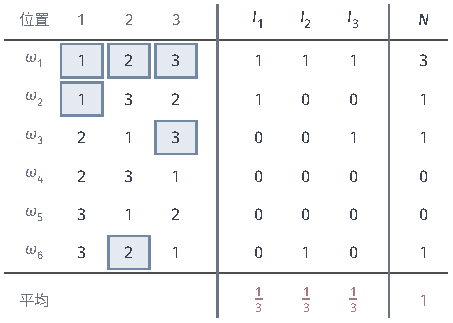
\includegraphics[width=77mm]{figures/07-probability/01-elementary-probability/tikz/rvm-fixed-points/figure.pdf}
 \caption{三封信装入三个信封的六种等可能方式。每行列出各位置装入的信，蓝框表示装对。$I_j$记录第$j$封是否装对，$N=I_1+I_2+I_3$。各列平均（红）满足$\tfrac13+\tfrac13+\tfrac13=1$，尽管$I_1,I_2,I_3$相互依赖。}
 \label{fig:rvm-fixed-points}
\end{BookInlineFigure}

\paragraph{乘积与无穷和}
线性性只涉及加法和数乘。乘积的期望一般不能拆开：取$Y=X$为奖金，则
\[
 \mathbb{E}[XY]=\mathbb{E}[X^{2}]=0\times\tfrac12+9\times\tfrac13+36\times\tfrac16=9,
\]
而$\mathbb{E}[X]\,\mathbb{E}[Y]=4$。乘积可以拆开的充分条件是独立，这需要联合分布，在第~\ref{chap:random-vectors}章讨论。

线性性对有限个变量成立。对无穷多个变量之和，等式
\[
 \mathbb{E}\Bigl[\sum_{k=1}^{\infty}X_k\Bigr]=\sum_{k=1}^{\infty}\mathbb{E}[X_k]
\]
相当于交换求和与取极限的次序，需要非负性或绝对可和这样的额外条件。这类交换的一般依据在第~\ref{chap:probability-spaces}章由积分的收敛定理给出。

\subsection{函数的期望}
\label{sec:rvm-function-expectation}

奖金的平方平均是多少？按定义，应当先求出新变量$Y=X^{2}$的概率表：$Y$取$0,9,36$，概率依次为$\tfrac12,\tfrac13,\tfrac16$，再加权得$9$。上一小节正是这样做的。但这个结果也可以不写出$Y$的分布，直接在$X$的每个取值上计算$x^{2}$再加权。下面的定理说明这种直接计算总是正确的，只要相应的和或积分绝对收敛。

\begin{theorem}[函数的期望]
\label{thm:rvm-lotus}
设$g$是实值函数。
\begin{enumerate}
 \item 若$X$离散，取值$x_i$，且$\sum_i\lvert g(x_i)\rvert\,p_X(x_i)<\infty$，则$g(X)$可积，且
 \begin{equation}
  \mathbb{E}[g(X)]=\sum_{i}g(x_i)\,p_X(x_i) .
  \label{eq:rvm-lotus-discrete}
 \end{equation}
 \item 若$X$有密度$f_X$，$g$分段连续，且$\int_{-\infty}^{\infty}\lvert g(x)\rvert f_X(x)\,\mathrm{d}x<\infty$，则$g(X)$可积，且
 \begin{equation}
  \mathbb{E}[g(X)]=\int_{-\infty}^{\infty}g(x)\,f_X(x)\,\mathrm{d}x .
  \label{eq:rvm-lotus-density}
 \end{equation}
\end{enumerate}
若$g\geq0$，两式在不要求有限的情况下也成立，两边同时为有限数或同时为$+\infty$。
\end{theorem}

\begin{proof}
离散情形。$Y=g(X)$的取值是集合$\{g(x_i)\}$中的数。对每个$y$，事件$\{Y=y\}$是若干个事件$\{X=x_i\}$（$g(x_i)=y$）的并，所以
\[
 p_Y(y)=\sum_{i:\,g(x_i)=y}p_X(x_i) .
\]
代入$Y$的期望，再把对$y$与对$i$的二重和合并成对$i$的一重和，得到
\[
 \sum_{y}y\,p_Y(y)=\sum_{y}\sum_{i:\,g(x_i)=y}g(x_i)\,p_X(x_i)=\sum_{i}g(x_i)\,p_X(x_i) .
\]
最后一步中每个$i$恰好出现在$y=g(x_i)$那一组。对$\lvert g\rvert$作同样的计算，得到
\[
 \mathbb{E}\lvert Y\rvert=\sum_i\lvert g(x_i)\rvert\,p_X(x_i)<\infty,
\]
所以$Y$可积，而绝对收敛保证了上面的重新分组不改变和。$g\geq0$时各项非负，重新分组同样不改变和，结论对$+\infty$也成立。

密度情形只证$g$在$X$的取值区间$(\alpha,\beta)$上连续可微且$g'>0$的情形。这时$g$把$(\alpha,\beta)$一一映成区间$(g(\alpha^{+}),g(\beta^{-}))$，记反函数为$h$。由$\{g(X)\leq y\}=\{X\leq h(y)\}$，
\[
 F_Y(y)=F_X\bigl(h(y)\bigr),\qquad f_Y(y)=f_X\bigl(h(y)\bigr)\,h'(y) .
\]
先设$g\geq0$。在$\int y\,f_Y(y)\,\mathrm{d}y$中作换元$y=g(x)$，$h(y)=x$，$\mathrm{d}y=g'(x)\,\mathrm{d}x$，并利用$h'(g(x))g'(x)=1$，得到
\[
 \int y\,f_X\bigl(h(y)\bigr)h'(y)\,\mathrm{d}y=\int_{\alpha}^{\beta}g(x)\,f_X(x)\,\mathrm{d}x .
\]
被积函数非负，反常积分的换元对有限值和$+\infty$都成立。一般的$g$对正部$g^{+}$与负部$g^{-}$分别使用这一结论再相减。$g'<0$时换元会交换积分上下限，结论相同。
\end{proof}

密度情形的一般证明需要先求出$g(X)$的分布，而$g(X)$可能根本没有密度，例如$g$是指示函数或在某个区间上为常数。第~\ref{chap:random-variable-transformations}章用换元公式处理分段单调的$g$，第~\ref{chap:probability-spaces}章把式~\eqref{eq:rvm-lotus-density}作为推前分布上的积分一般地证明。在这之前，我们在定理的条件下使用它。

定理中的绝对可积条件要对每个$g$分别检查，它与$X$本身是否可积无关。例如密度$f_X(x)=x^{-2}$（$x\geq1$）的$X$满足
\[
 \mathbb{E}[X]=\int_1^{\infty}x\cdot x^{-2}\,\mathrm{d}x=+\infty,
\]
但
\[
 \mathbb{E}\bigl[\sqrt{X}\bigr]=\int_1^{\infty}x^{1/2}\cdot x^{-2}\,\mathrm{d}x=\int_1^{\infty}x^{-3/2}\,\mathrm{d}x=2,
\]
增长较慢的函数仍可积。反过来，$X$可积也不保证$X^{2}$可积，第~\ref{sec:rvm-moments}节会系统地讨论这一点。

\paragraph{指示函数：概率也是期望}
取$g=\mathbf{1}_{A}$，它在$x\in A$时为$1$，否则为$0$。式~\eqref{eq:rvm-lotus-discrete}或式~\eqref{eq:rvm-lotus-density}的右边只剩下$A$上的质量，于是
\begin{equation}
 \mathbb{E}\bigl[\mathbf{1}_{A}(X)\bigr]=\mathbb{P}(X\in A) .
 \label{eq:rvm-indicator}
\end{equation}
概率因此是期望的特殊情形，信封例子中$\mathbb{E}[I_j]=\tfrac13$用的正是这一点。对奖金表取$A=(0,\infty)$，得到中奖的概率$\tfrac13+\tfrac16=\tfrac12$。

\paragraph{收益：不必先求新变量的分布}
奖金本身就是点数的函数。设$D$是骰子点数，$g(1)=g(2)=g(3)=0$，$g(4)=g(5)=3$，$g(6)=6$，则$X=g(D)$。由式~\eqref{eq:rvm-lotus-discrete}，
\[
 \mathbb{E}[g(D)]=\tfrac16\bigl(g(1)+\dots+g(6)\bigr)=\tfrac16(0+0+0+3+3+6)=2,
\]
与先求$X$的概率表再加权的结果相同。若参加一次要付$2.5$元，净收益是$g(D)-2.5$，由线性性它的期望是$-0.5$元，长期参加平均每次亏$0.5$元。

连续的例子也一样。设$X$的密度是$2x$（$0<x<1$），$Y=X^{2}$。直接计算
\[
 \mathbb{E}[X^{2}]=\int_0^1x^{2}\cdot2x\,\mathrm{d}x=\tfrac12 .
\]
另一方面，对$0<y<1$有
\[
 F_Y(y)=\mathbb{P}(X\leq\sqrt{y})=\int_0^{\sqrt{y}}2x\,\mathrm{d}x=y,
\]
所以$Y$在$(0,1)$上有常数密度$1$，$\mathbb{E}[Y]=\int_0^1y\,\mathrm{d}y=\tfrac12$。两条途径对应图~\ref{fig:rvm-square-transform}中两块面积，它们相等。

\begin{BookInlineFigure}
 \centering
 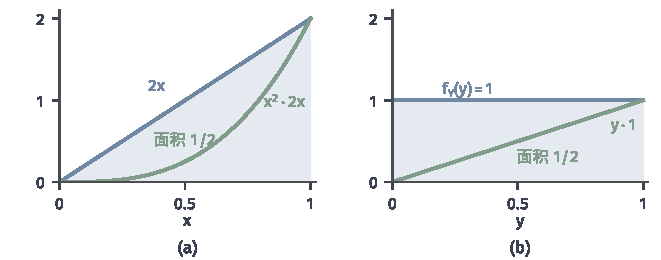
\includegraphics[width=112mm]{figures/07-probability/01-elementary-probability/matplotlib/rvm-square-transform/figure.pdf}
 \caption{用两种方式计算$\mathbb{E}[X^{2}]$，$X$的密度为$2x$。(a)在$X$的尺度上积分$x^{2}\cdot2x$（绿色曲线下的面积）；(b)先求出$Y=X^{2}$的密度$f_Y(y)=1$，再积分$y\cdot1$（绿色直线下的面积）。两块面积都是$1/2$。}
 \label{fig:rvm-square-transform}
\end{BookInlineFigure}

\paragraph{平方误差与绝对误差}
如果要用一个常数$c$预测奖金，平方误差的平均是多少？设$\mathbb{E}[X^{2}]<\infty$，记$\mu=\mathbb{E}[X]$。把$X-c$写成$(X-\mu)+(\mu-c)$后展开，由线性性，交叉项的期望是$2(\mu-c)\,\mathbb{E}[X-\mu]=0$，于是
\begin{equation}
 \mathbb{E}\bigl[(X-c)^{2}\bigr]=\mathbb{E}\bigl[(X-\mu)^{2}\bigr]+(\mu-c)^{2} .
 \label{eq:rvm-square-error}
\end{equation}
右边第二项只在$c=\mu$时为零，所以期望是平方误差意义下最好的常数预测。对奖金表，偏差$X-2$取$-2,1,4$，
\[
 \mathbb{E}\bigl[(X-2)^{2}\bigr]=4\cdot\tfrac12+1\cdot\tfrac13+16\cdot\tfrac16=5,
\]
因此
\[
 \mathbb{E}\bigl[(X-c)^{2}\bigr]=5+(c-2)^{2},
\]
它是图~\ref{fig:rvm-error-curves}(a)中的抛物线，最低点为$(2,5)$。最小值$5$是下一节的方差。

把平方换成绝对值，结论就变了。对奖金表，
\[
 \mathbb{E}\lvert X-c\rvert=\tfrac12\lvert c\rvert+\tfrac13\lvert3-c\rvert+\tfrac16\lvert6-c\rvert .
\]
逐段去掉绝对值：$c<0$时它等于$2-c$，$0\leq c\leq3$时等于常数$2$，$3\leq c\leq6$时等于$\tfrac23c$，$c>6$时等于$c-2$。最小值在整个区间$[0,3]$上取到。这个区间正是使$\mathbb{P}(X\leq c)\geq\tfrac12$且$\mathbb{P}(X\geq c)\geq\tfrac12$的点，即奖金的全部中位数。

\begin{BookInlineFigure}
 \centering
 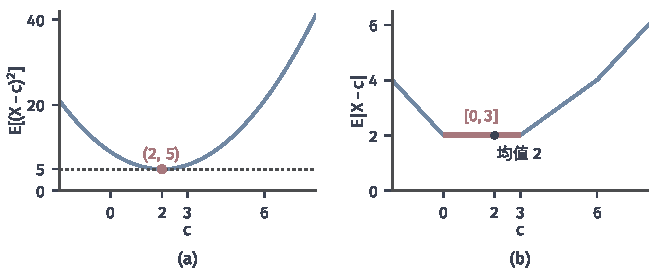
\includegraphics[width=112mm]{figures/07-probability/01-elementary-probability/matplotlib/rvm-error-curves/figure.pdf}
 \caption{用常数$c$预测奖金$X$的平均误差。(a)平方误差$\mathbb{E}[(X-c)^{2}]=5+(c-2)^{2}$在均值$c=2$处取最小值$5$（红点）。(b)绝对误差$\mathbb{E}\lvert X-c\rvert$是折线，在中位数构成的区间$[0,3]$（红色粗线）上取最小值$2$，均值$2$（黑点）恰好也在其中。}
 \label{fig:rvm-error-curves}
\end{BookInlineFigure}

图~\ref{fig:rvm-error-curves}(b)的斜率解释了原因：当$c$不是取值点时，$c$右移一个单位，左侧质量$\mathbb{P}(X<c)$的误差各增加一，右侧质量$\mathbb{P}(X>c)$的误差各减少一，斜率是$\mathbb{P}(X<c)-\mathbb{P}(X>c)$。左右质量相等时斜率为零，这就是中位数的条件。均值与中位数因此回答不同的问题：均值使平方误差最小，受远处取值的影响大；中位数使绝对误差最小，只看质量在左右两侧的分配。若把奖金$6$换成$60$，均值从$2$变成$11$，中位数区间仍是$[0,3]$。

\subsection{凸函数的期望}
\label{sec:rvm-convex-expectation}

先平均再平方，与先平方再平均，结果一样吗？对奖金表，$(\mathbb{E}[X])^{2}=4$，而$\mathbb{E}[X^{2}]=9$。一般地，对非线性函数$f$，$\mathbb{E}[f(X)]$与$f(\mathbb{E}[X])$不相等，但对凸函数两者总有确定的大小关系。这个关系在后面比较风险、比较信息量时反复使用。

\paragraph{有限加权平均}
回忆凸函数的定义：区间$I$上的$f$对一切$x,y\in I$与$\lambda\in[0,1]$满足
\[
 f\bigl(\lambda x+(1-\lambda)y\bigr)\leq\lambda f(x)+(1-\lambda)f(y),
\]
即两点间的图像不高于弦，可参考\BookChapterRef{chap:univariate-differentiation}{卷一第6章“一元函数的微分”}。两点的情形推广到有限个点，就得到下面的引理。

\begin{lemma}[有限加权平均的凸性]
\label{lem:rvm-jensen-finite}
设$f$是区间$I$上的凸函数，点$x_1,\dots,x_n$都在$I$中，权重$\lambda_1,\dots,\lambda_n$非负且和为一。则
\begin{equation}
 f\Bigl(\sum_{i=1}^{n}\lambda_ix_i\Bigr)\leq\sum_{i=1}^{n}\lambda_if(x_i) .
 \label{eq:rvm-jensen-finite}
\end{equation}
\end{lemma}

\begin{proof}
对$n$归纳。$n=1$时两边相等，$n=2$时就是凸函数的定义。设结论对$n-1$个点成立。若$\lambda_n=1$，其余权重都为零，结论成立。否则记$s=1-\lambda_n>0$，令
\[
 \bar{x}=\sum_{i=1}^{n-1}\frac{\lambda_i}{s}x_i .
\]
权重$\lambda_i/s$非负且和为一，$\bar{x}$是$I$中点的加权平均，仍在区间$I$中，并且$\sum_{i}\lambda_ix_i=s\bar{x}+\lambda_nx_n$。先用两点的凸性，再对$\bar{x}$用归纳假设，得到
\[
 f\bigl(s\bar{x}+\lambda_nx_n\bigr)\leq sf(\bar{x})+\lambda_nf(x_n)\leq s\sum_{i=1}^{n-1}\frac{\lambda_i}{s}f(x_i)+\lambda_nf(x_n),
\]
右边等于$\sum_{i=1}^{n}\lambda_if(x_i)$。
\end{proof}

引理有一个直观的重心解释。把质量$\lambda_i$放在图像上的点$(x_i,f(x_i))$，这组质量的重心是$\bigl(\sum\lambda_ix_i,\sum\lambda_if(x_i)\bigr)$，它落在这些点的凸包内。凸函数的图像向下弯，凸包整个位于图像上方或图像上，所以重心的高度不低于图像在同一横坐标处的高度。图~\ref{fig:rvm-jensen}(a)用奖金表画出了这一点：三个点$(0,0)$、$(3,9)$、$(6,36)$的重心是$(2,9)$，图像在$x=2$处的高度只有$4$。

\paragraph{支撑线}
推广到可数个取值和密度时，不能再逐点归纳，需要另一个工具：在凸函数图像上任一内点处，总可以放一条不高于图像的直线。

\begin{lemma}[凸函数的支撑线]
\label{lem:rvm-support-line}
设$f$是开区间$I$上的凸函数，$m\in I$。存在实数$s$，使对一切$x\in I$，
\begin{equation}
 f(x)\geq f(m)+s(x-m) .
 \label{eq:rvm-support-line}
\end{equation}
若$f$在$m$处可微，可取$s=f'(m)$。若$f$严格凸，则$x\neq m$时不等式严格成立。
\end{lemma}

\begin{proof}
取$x<m<y$，均在$I$中。把$m$写成$x$与$y$的凸组合，由凸性得到弦的斜率关系
\[
 \frac{f(m)-f(x)}{m-x}\leq\frac{f(y)-f(m)}{y-m},
\]
这正是上面所引可微凸函数刻画的证明第一步，那一步没有用到可微性。上式对一切$x<m$与$y>m$成立，所以左边对$x$的上确界$L$不超过右边对$y$的下确界$R$，两者都是有限数。取$s\in[L,R]$。对$x<m$，由$\frac{f(m)-f(x)}{m-x}\leq s$得$f(x)\geq f(m)+s(x-m)$；对$y>m$，由$\frac{f(y)-f(m)}{y-m}\geq s$得同一不等式。可微时左右两侧的斜率都趋于$f'(m)$，所以$L=R=f'(m)$。

若$f$严格凸，假设某个$x\neq m$使等号成立，不妨设$x>m$。$f$在$x$与$m$处都与直线$\ell(t)=f(m)+s(t-m)$相等，取中点$z=(x+m)/2$，严格凸性给出$f(z)<\frac12f(m)+\frac12f(x)=\ell(z)$，与$f\geq\ell$矛盾。
\end{proof}

\paragraph{Jensen不等式}
有了支撑线，在$m=\mathbb{E}[X]$处放一条支撑线再取期望，就得到对一般随机变量成立的不等式。

\begin{theorem}[Jensen不等式]
\label{thm:rvm-jensen}
设$f$是开区间$I$上的凸函数，$X$的取值都在$I$中，$X$与$f(X)$都可积。则$\mathbb{E}[X]\in I$，且
\begin{equation}
 f\bigl(\mathbb{E}[X]\bigr)\leq\mathbb{E}\bigl[f(X)\bigr] .
 \label{eq:rvm-jensen}
\end{equation}
若$f$严格凸，等号成立当且仅当$X$以概率一等于常数$\mathbb{E}[X]$。
\end{theorem}

\begin{proof}
先说明$m=\mathbb{E}[X]$在$I$中。设$I$的左端点$\alpha$有限，$X-\alpha$的取值都为正。离散时，$\mathbb{E}[X]-\alpha=\sum_i(x_i-\alpha)p_X(x_i)$中各项非负且总有正项；有密度时，被积函数$(x-\alpha)f_X(x)$非负，且$X$落在某个$[\alpha+\delta,\infty)$中的概率为正，于是积分至少是$\delta$乘这个概率。两种情形都有$m>\alpha$。右端点同理，所以$m\in I$。

由引理~\ref{lem:rvm-support-line}，存在$s$使$f(x)\geq f(m)+s(x-m)$对一切$x\in I$成立。把$x$换成$X$，两边都是可积的随机变量，由保序性与线性性，
\[
 \mathbb{E}[f(X)]\geq f(m)+s\bigl(\mathbb{E}[X]-m\bigr)=f(m) .
\]

等号情形。记$D(x)=f(x)-f(m)-s(x-m)\geq0$，则$\mathbb{E}[D(X)]=\mathbb{E}[f(X)]-f(m)$。$f$严格凸时，$x\neq m$有$D(x)>0$。若$X$离散且$\mathbb{P}(X\neq m)>0$，和式$\sum_iD(x_i)\,p_X(x_i)$中有正项，所以$\mathbb{E}[D(X)]>0$。若$X$有密度，单点$m$的概率为零，总可以找到一个不含$m$的闭区间，使$X$落在其中的概率为正；凸函数在开区间上连续，$D$在这个闭区间上有正的最小值，于是$\mathbb{E}[D(X)]>0$。反过来，$X$以概率一等于$m$时$f(X)$以概率一等于$f(m)$，两边相等。
\end{proof}

定理的条件各有用处。区间取开区间，是为了让$m$成为内点，从而支撑线存在；在闭区间的端点处，凸函数可能没有有限斜率的支撑线，例如$-\sqrt{x}$在$0$处。$X$与$f(X)$可积，保证了取期望时两边都是有限数并可以用线性性。若$f(X)$只是非负而期望为$+\infty$，不等式按$+\infty$理解仍然成立。

\begin{BookInlineFigure}
 \centering
 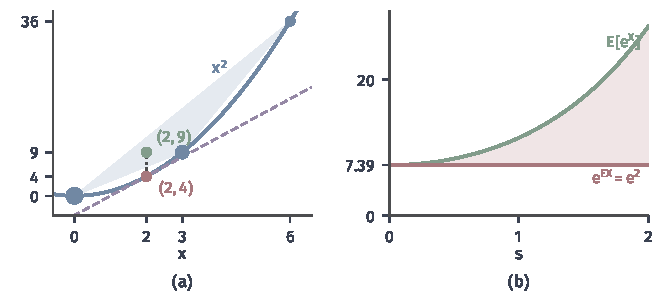
\includegraphics[width=112mm]{figures/07-probability/01-elementary-probability/matplotlib/rvm-jensen/figure.pdf}
 \caption{Jensen不等式的几何。(a)$f(x)=x^{2}$与奖金表：蓝点$(x_i,x_i^{2})$按概率大小画出，浅蓝三角是它们的凸包，重心$(\mathbb{E}[X],\mathbb{E}[X^{2}])=(2,9)$（绿）高于$(2,f(2))=(2,4)$（红）；紫色虚线是$x=2$处的支撑线$y=4+4(x-2)$。(b)$X$以各$\tfrac12$的概率取$2\pm s$时，$\mathbb{E}[\mathrm{e}^{X}]=\mathrm{e}^{2}\cosh s$（绿）与$\mathrm{e}^{\mathbb{E}[X]}=\mathrm{e}^{2}$（红）之差（浅红）随$s$增大。}
 \label{fig:rvm-jensen}
\end{BookInlineFigure}

\paragraph{平方、指数与对数}
取$f(x)=x^{2}$，它在$\mathbb{R}$上严格凸，Jensen不等式给出$(\mathbb{E}[X])^{2}\leq\mathbb{E}[X^{2}]$。差值$\mathbb{E}[X^{2}]-(\mathbb{E}[X])^{2}$就是式~\eqref{eq:rvm-square-error}中$c=0$时多出的那一项$\mathbb{E}[(X-\mu)^{2}]$，它衡量$X$偏离均值的程度。奖金表的差值是$9-4=5$。

取$f(x)=\mathrm{e}^{x}$。对密度$2x$，分部积分得
\[
 \mathbb{E}[\mathrm{e}^{X}]=\int_0^12x\,\mathrm{e}^{x}\,\mathrm{d}x=\Bigl[2(x-1)\mathrm{e}^{x}\Bigr]_0^1=2,
\]
而$\mathrm{e}^{2/3}\approx1.948$，差值只有约$0.05$。差值小，是因为$X$集中在长度为$1$的区间里，指数函数在这么短的区间上接近一条直线。图~\ref{fig:rvm-jensen}(b)取两点分布$2\pm s$，差值$\mathrm{e}^{2}(\cosh s-1)$随分散程度$s$迅速增大：变量越分散，凸函数的弯曲被平均放大得越多。

对凹函数，不等号反向。$\ln x$在$(0,\infty)$上严格凹，所以$\mathbb{E}[\ln X]\leq\ln\mathbb{E}[X]$。对密度$2x$，
\[
 \mathbb{E}[\ln X]=\int_0^12x\ln x\,\mathrm{d}x=\Bigl[x^{2}\ln x-\tfrac{x^{2}}{2}\Bigr]_0^1=-\tfrac12,
\]
而$\ln\tfrac23\approx-0.405$，确实更大。第~\ref{chap:information-measures}章研究信息量时，正是用对数的凹性证明各种信息量非负。

\paragraph{不是凸函数时}
若$f$既不凸也不凹，两边的大小关系由分布决定。取$f(x)=x^{3}$。奖金表给出
\[
 \mathbb{E}[X^{3}]=27\cdot\tfrac13+216\cdot\tfrac16=45>2^{3}=8 .
\]
把奖金变号，$-X$的三次方平均是$-45$，小于$(-2)^{3}=-8$。以各$\tfrac12$的概率取$\pm1$时两边都是$0$。所以Jensen不等式中凸性不能省略，它决定了不等号的方向。
